\documentclass{beamer}
\usepackage{graphicx}
\usepackage{xmpmulti} 
\usepackage{subfig}

\usetheme{Frankfurt}
\title{Applying Spectral Graph Theory to Microbial Analysis}
\author{Zain Jabbar, Monique Chyba}

\begin{document}

\maketitle
 
\section{Introduce Myself}
\section{Central Question / Motivation}
\begin{frame}{The Importance of the Microbiome}
  \centering \includegraphics[width=0.85\textwidth]{fatmouse.jpg}
\end{frame}

\begin{frame}{Waimea Valley}
  \centering 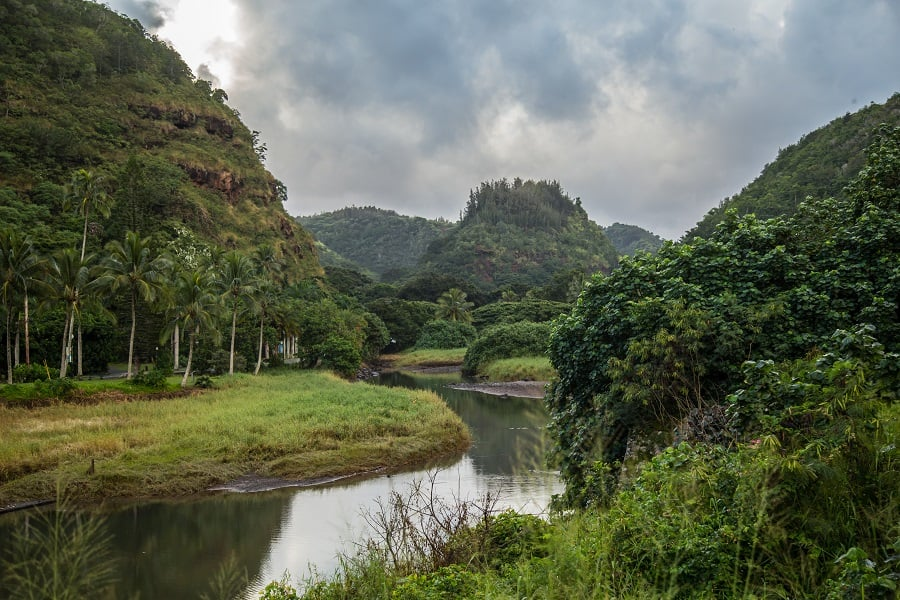
\includegraphics[width=0.85\textwidth]{waimea.jpg}
\end{frame}

\begin{frame}{The Data}
\begin{figure}%
    \centering
    \subfloat[\centering Abundance Table]{{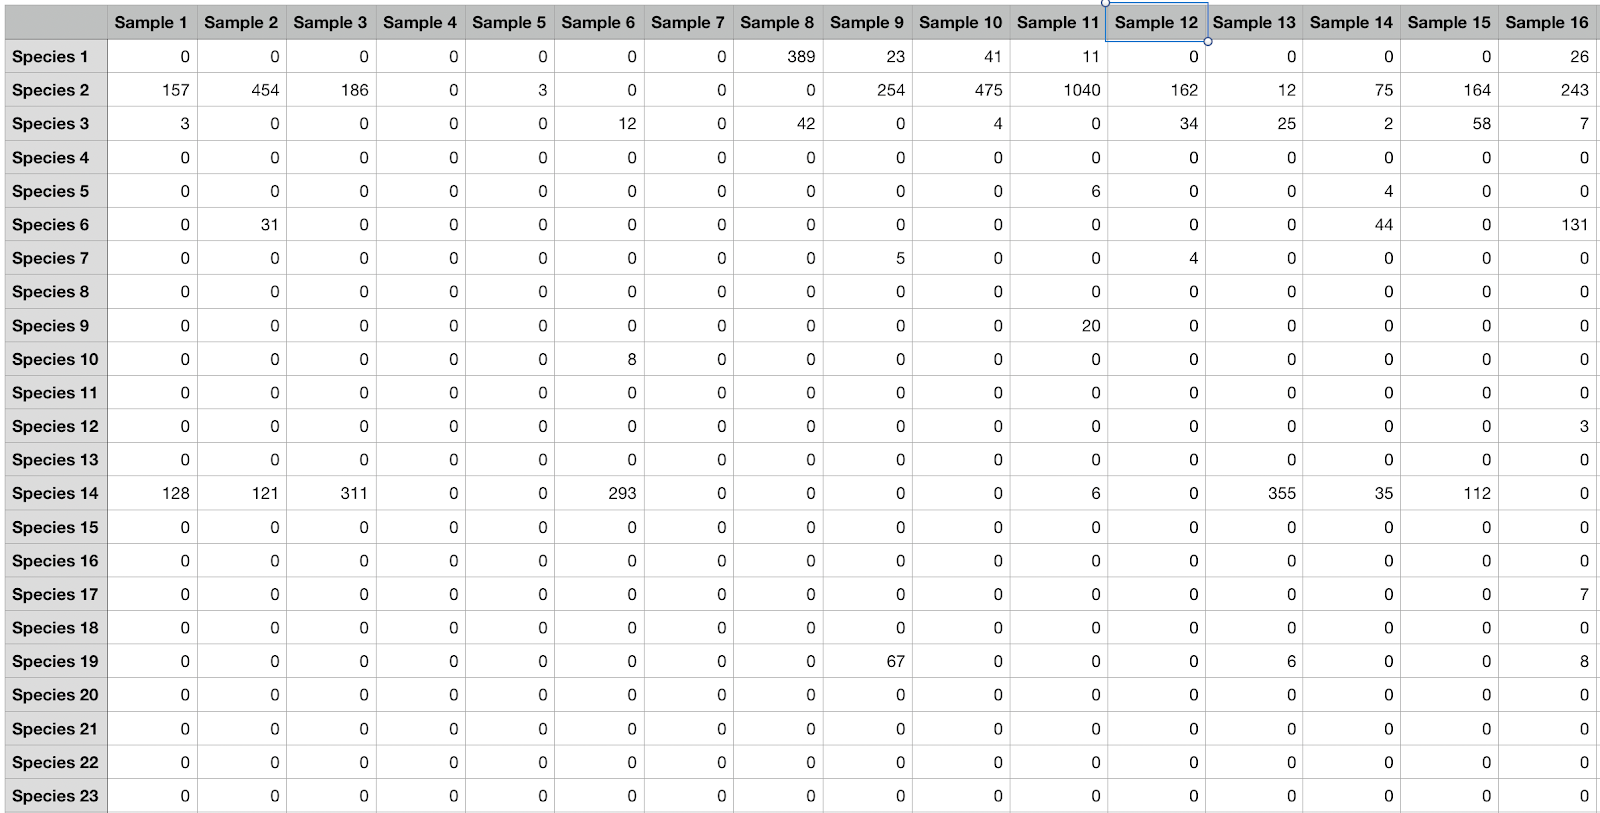
\includegraphics[width=8cm]{abundance.png}}}%
    \qquad
    \subfloat[\centering Metadata]{{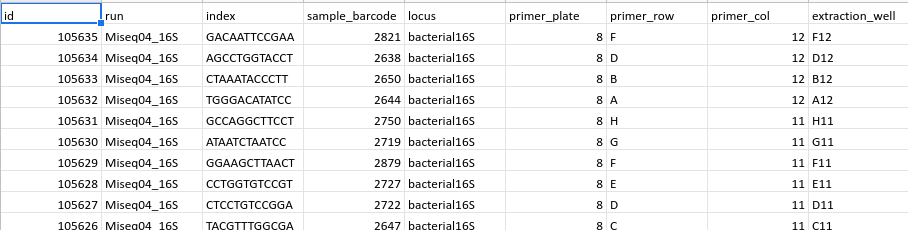
\includegraphics[width=8cm]{metadata.png}}}%
    \label{fig:example}%
\end{figure}
\end{frame}

\begin{frame}{Problem Statement}
  \centering Explore!
\end{frame}

\begin{frame}{Previous Microbiology Work}
  \begin{figure}%
    \centering 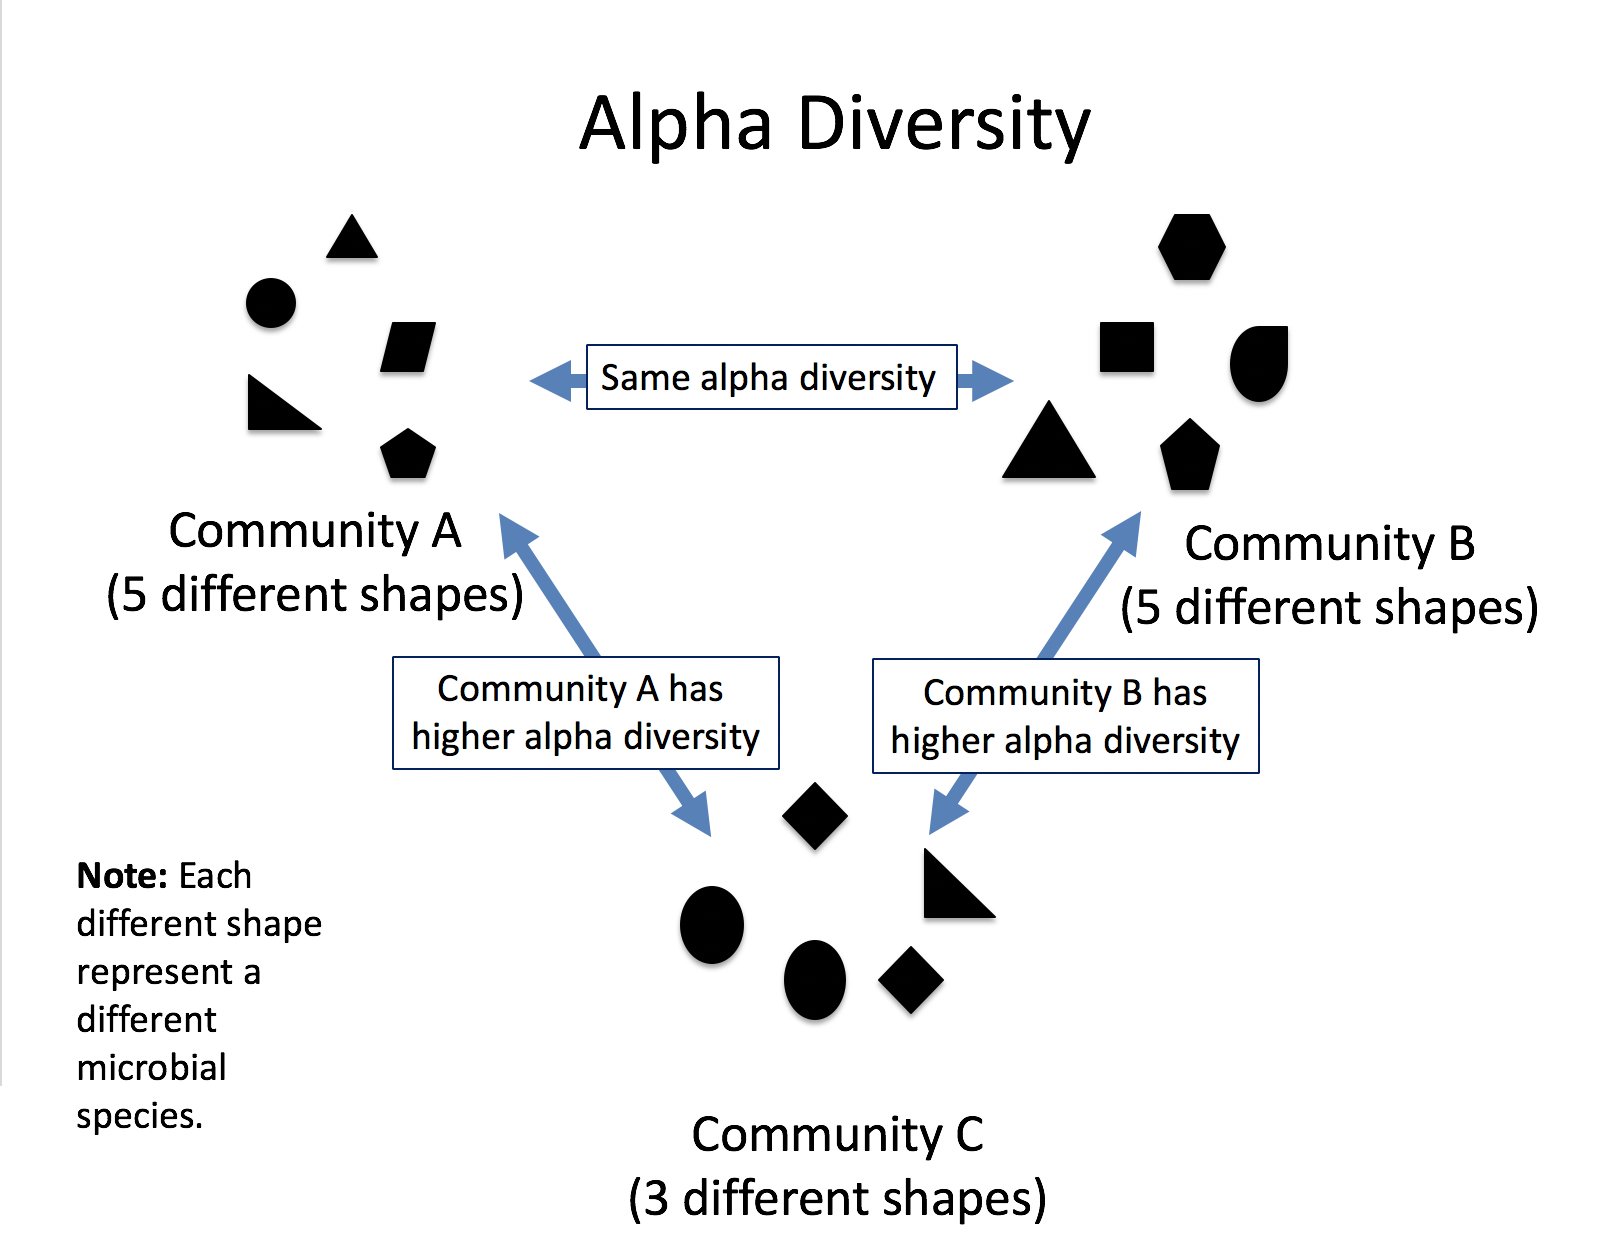
\includegraphics[width=0.75\textwidth]{diversity.png}
  \end{figure}
\end{frame}
 
\section{Background}
\begin{frame}{Manifolds}
    \begin{figure}%
    \centering 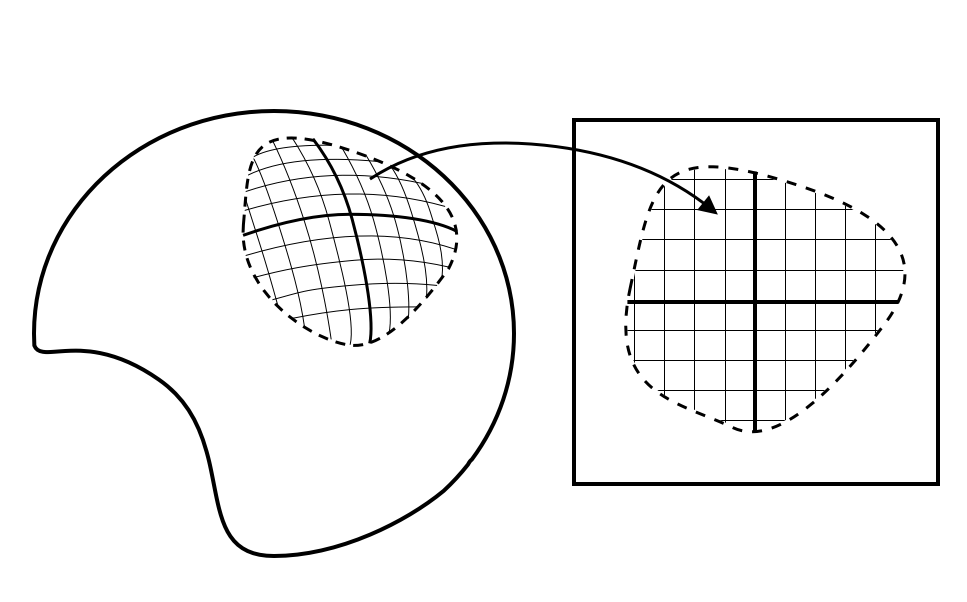
\includegraphics[width=0.75\textwidth]{manifold_general.png}
  \end{figure} 
\end{frame}    

\begin{frame}{Graphs}
  \begin{figure}%
    \centering
    \subfloat[\centering Graphs in General]{{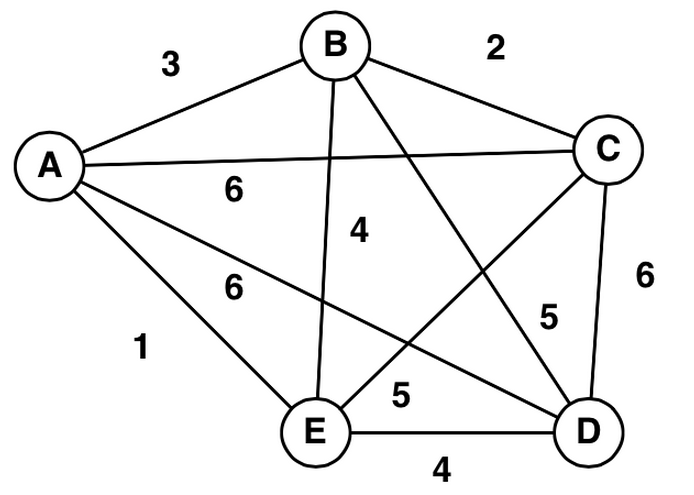
\includegraphics[width=5cm]{graph_general.png}}}%
    \qquad
    \subfloat[\centering Graphs as Manifolds]{{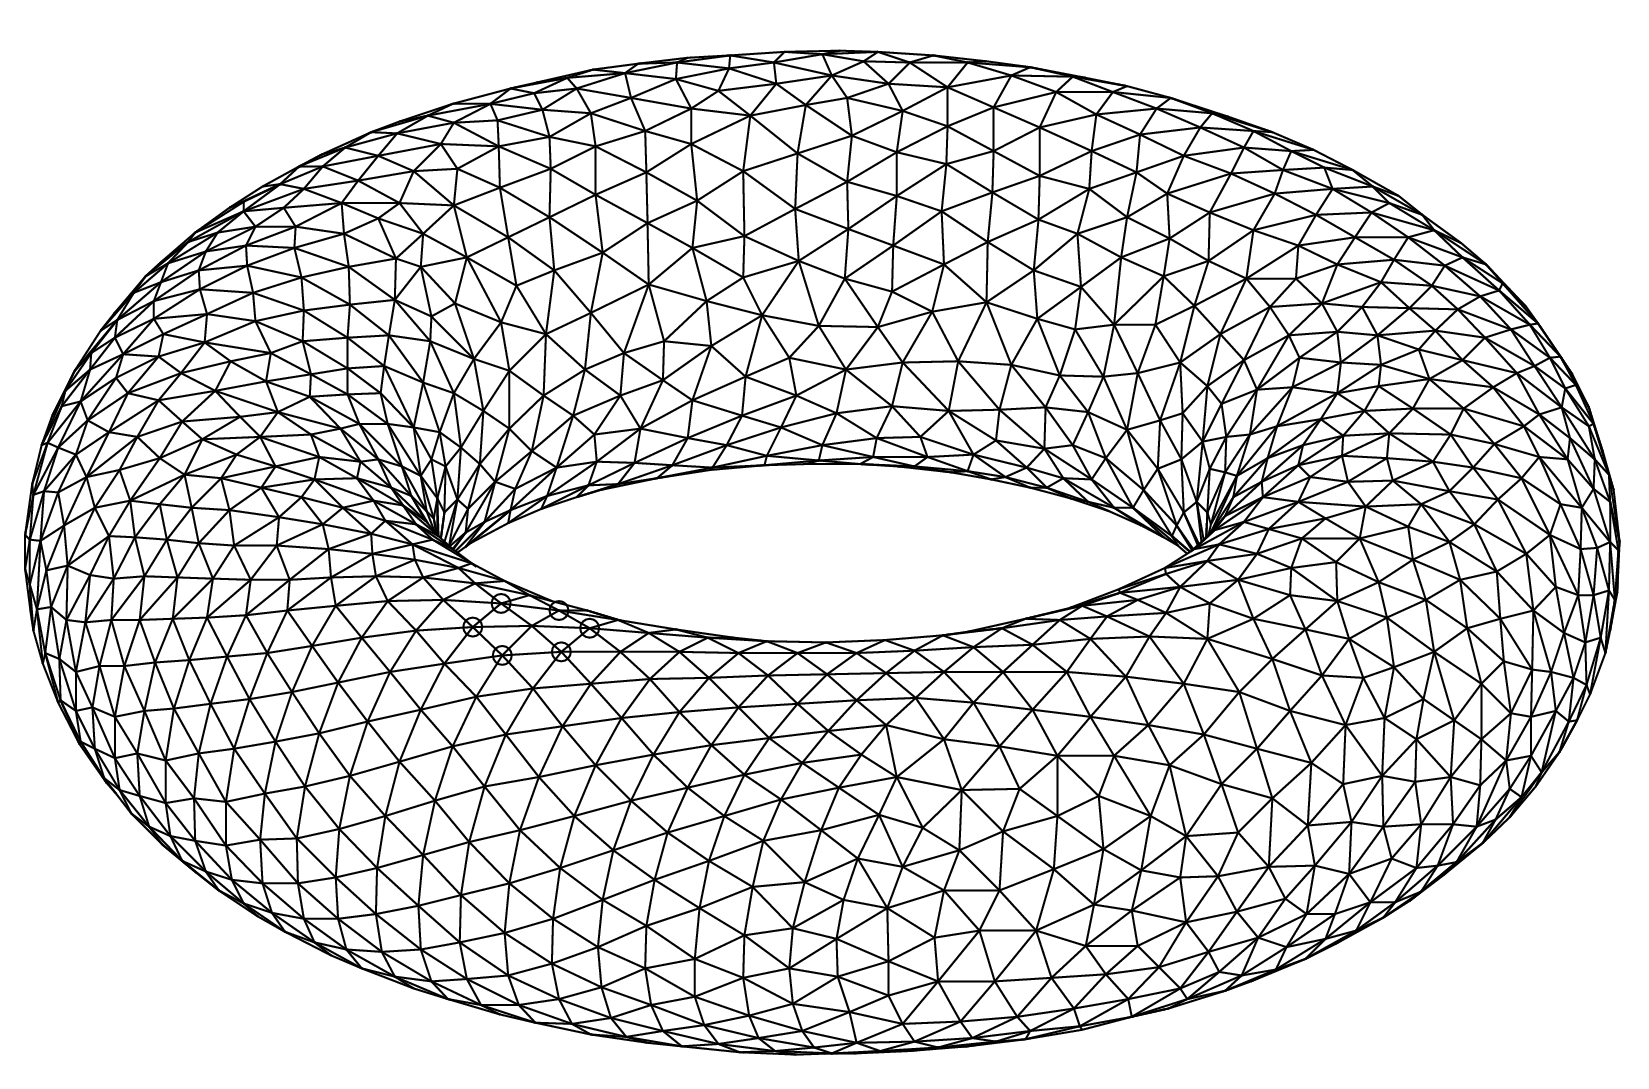
\includegraphics[width=5cm]{graph_as_manifold.png}}}%
    \label{fig:example}%
\end{figure}  
\end{frame} 

\section{Methodology}

\begin{frame}{Compute Adjacency Matrix}
    \centering 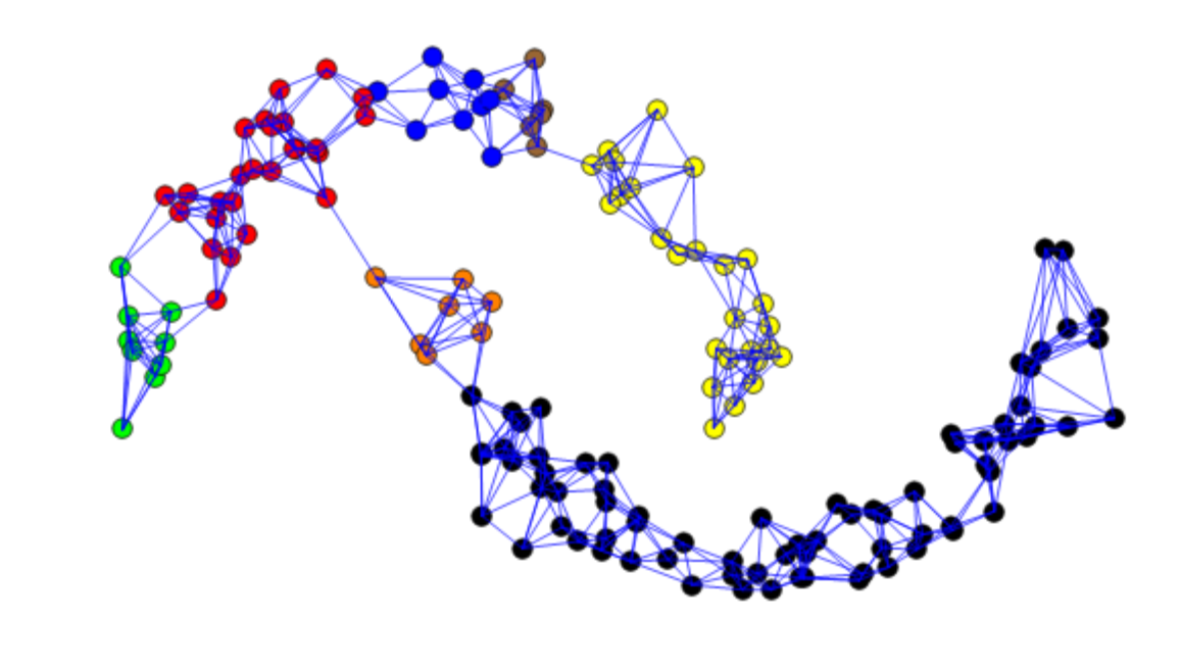
\includegraphics[width=0.75\textwidth]{K7Nearest.png}
\end{frame}

\begin{frame}{Compute Graph Laplacian and Eigenvalues} 
\centering\multiinclude[format=png, graphics={width=\textwidth}]{gif/laplacian}
\end{frame}
 
\section{Results} 
\begin{frame}
  \begin{figure}
\begin{center}
  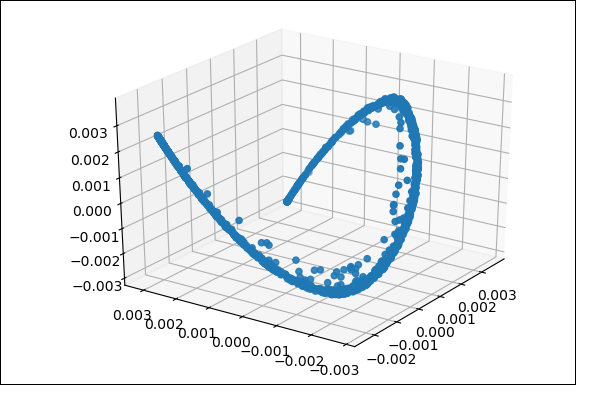
\includegraphics[width=.45\linewidth]{view1.png}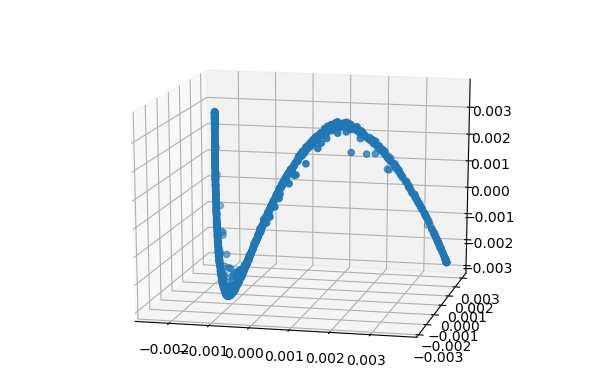
\includegraphics[width=.5\linewidth]{view2.png}
  \caption{The plots are a representation of the dimensionality reduction procedure and display a one dimensional submanifold in $\mathbb{R}^3$.}
   \label{fig:data_curve}
  \end{center}
\end{figure}
\end{frame}

\begin{frame}
  \begin{figure}
\begin{center}
  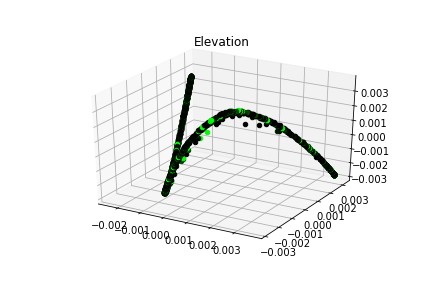
\includegraphics[width=.40\linewidth]{elevation.png}\\
  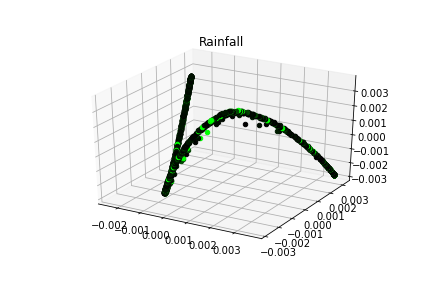
\includegraphics[width=.40\linewidth]{rainfall.png}\\
  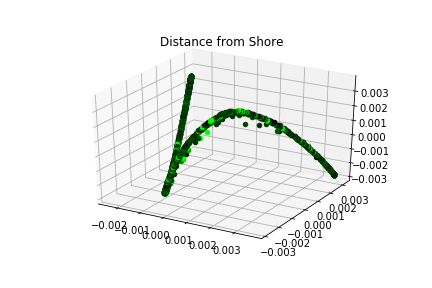
\includegraphics[width=.40\linewidth]{distance_from_shore.png}
   \label{fig:data_curve}
  \end{center}
\end{figure}
\end{frame}

\section{Thank Audience + Q and A}

\begin{frame}
  \centering Thank you for listening!
\end{frame}

\end{document}
 
